\documentclass[10pt,twocolumn]{article}
\usepackage[a4paper,margin=1.9cm,columnsep=0.7cm,top=2.3cm,bottom=2.2cm]{geometry}
\usepackage[T1]{fontenc}
\usepackage{newtxtext,newtxmath}
\usepackage{microtype}
\usepackage{booktabs,tabularx,array}
\usepackage{xcolor}
\usepackage{tikz}
\usetikzlibrary{arrows.meta,positioning,calc}
\usepackage{fancyhdr}
\usepackage[font=small,labelfont=bf]{caption}
\usepackage{titlesec}
\usepackage[colorlinks=true,linkcolor=black,citecolor=black,urlcolor=black]{hyperref}

\definecolor{lilac}{HTML}{7C5CE0}
\definecolor{teal}{HTML}{0B8A77}
\definecolor{amber}{HTML}{B45F12}
\definecolor{ink}{HTML}{17130D}
\definecolor{mute}{HTML}{6B6456}

\titleformat{\section}{\normalfont\large\bfseries}{\thesection}{0.6em}{}
\titleformat{\subsection}{\normalfont\normalsize\bfseries}{\thesubsection}{0.6em}{}
\titlespacing*{\section}{0pt}{1.1em}{0.4em}
\titlespacing*{\subsection}{0pt}{0.8em}{0.25em}

\pagestyle{fancy}
\fancyhf{}
\renewcommand{\headrulewidth}{0.3pt}
\fancyhead[L]{\small\color{mute} Bio-Inspired Agentic Swarms}
\fancyhead[R]{\small\color{amber}\textbf{DRAFT} \color{mute}--- first complete draft}
\fancyfoot[C]{\small\thepage}

\newcommand{\pending}[1]{\textcolor{amber}{[#1]}}
\newcolumntype{Y}{>{\raggedright\arraybackslash}X}
\setlength{\parskip}{0.25em}

\begin{document}

\twocolumn[
\begin{center}
{\LARGE\bfseries Bio-Inspired Agentic Swarms\par}
\vspace{0.35em}
{\Large\itshape Towards Leaderless AI\par}
\vspace{1.1em}
{\large Unfold --- AI Swarm Lab\par}
\vspace{0.2em}
{\small\texttt{unfold.host}\par}
\vspace{0.6em}
{\small\color{amber}\textbf{First complete draft, November 2026.} Not for circulation.\par}
\vspace{1.2em}
\begin{minipage}{0.86\textwidth}
\small
\textbf{Abstract.}
Systems of language-model agents are mostly built around a lead agent that reads the state of the work and assigns it to others. Living collectives coordinate without one: termites build, ants forage and bees choose a home through traces left in a shared environment and simple local rules. We offer a vocabulary for bringing those collectives into agent systems: five coordination \emph{primitives} (deposit, decay, threshold, quorum, recognition) defined as terms of one expression over a shared \emph{field}, and the notion of a \emph{regime} as a rule over that field. In this notation an orchestrator, a fixed schedule, one deep agent and a swarm coordinated through traces are points of the same space and can be compared. An atlas maps eight swarming collectives to mechanisms and to the class of problem each addresses, and states for each how little evidence there is that the analogue works with language-model agents. Reading ten neighbouring works from the papers themselves, we find shared-field coordination already built and scaled, but no comparison of one field-coordinated regime with another, with a fixed schedule, or with one agent holding the collective's budget. A preregistered pilot on one synthetic task makes those comparisons. Following traces beat a fixed schedule only when the budget did not cover the field and change was local (0.70 against 0.48); it lost when change was scattered or a trace was false; an orchestrator added nothing a rule did not; and no field-coordinated regime was above a single agent. On a public benchmark of real repositories, two agents that shared the work product as it was produced delivered both features in 0.38 of pairs, against 0.20 with messaging and 0.16 with no communication; one agent alone delivered 0.58. We do not claim that swarms are better. We claim that the question of when coordination without a leader pays can be asked precisely, and we show how.
\end{minipage}
\end{center}
\vspace{1.4em}
]

\section{Introduction}

The common way to build a system of several language-model agents is to put one of them in charge. A lead agent reads the request, decomposes it, assigns the parts to workers and assembles what comes back. The pattern is easy to reason about and it has a known weakness: everything passes through one context, the assignments are only as good as the lead's picture of the work, and that picture ages as the work changes. Taking the leader away and letting agents talk to each other does not remove the cost of coordinating. On real repositories, two agents that each implement one feature and can exchange messages succeed far less often than one agent that implements both, 0.28 against 0.48 for one frontier model, and messaging does not change the outcome~\cite{khatua2026}.

Living collectives solve problems of comparable shape with neither a leader nor conversation. A termite does not receive instructions; it responds to the state of the wall in front of it, and the wall coordinates the builders~\cite{grasse1959,theraulaz1999}. Ants find short paths because trails that are not reinforced evaporate~\cite{goss1989}. A honey bee swarm chooses a nest site through scouts that advertise, recruit and inhibit each other until enough of them are at one site~\cite{seeley2003,seeley2012}. In each case coordination is carried by a shared medium and by rules that an individual applies to what is in front of it.

Agent systems have begun to use the same idea. Agents have been made to coordinate through a shared artefact~\cite{rodriguez2026,pal2026}, and through a shared store in which messages gain weight when they are built upon and lose it with time, scaled to more than a hundred agents~\cite{qi2026}. What this work does not yet have is a common way to say what was built and against what it should be compared. Each system is one configuration of one mechanism, set against the baselines its authors chose; none is compared with another configuration, with a schedule that needs no coordination at all, or with a single agent given everything the collective spent (Section~\ref{sec:related}). The last comparison is the one now being asked of message-passing and orchestrated systems~\cite{fan2026,kim2025,gao2026}.

This paper asks when agent systems should be organised as leaderless collectives, and by which mechanism. It makes four contributions.

\begin{enumerate}\setlength{\itemsep}{0.1em}
\item \textbf{A notation.} Five primitives taken from natural collectives, defined as the terms of one expression over a shared field, and the notion of a regime as a rule over that field. An orchestrator, a fixed schedule, a single deep agent and field-coordinated swarms are written as points of one space (Section~\ref{sec:framework}).
\item \textbf{An atlas.} A table from swarming collectives to mechanism, to primitive, to the class of problem the mechanism addresses, with an inclusion rule and, for each row, the evidence that the analogue works with language-model agents (Section~\ref{sec:atlas}).
\item \textbf{A reading of neighbouring work.} Ten papers read from the source, with what each tests and leaves untested (Section~\ref{sec:related}).
\item \textbf{A pilot.} One synthetic task in four settings, preregistered, with every arm a point of the notation and the schedule, the orchestrator and the single agent present (Section~\ref{sec:pilot}).
\end{enumerate}

We state the outcome at the start, because it is not the one the title might suggest. Coordination through traces beat a fixed schedule in one of four settings, lost in two, and was unnecessary in the fourth. An orchestrator never did better than a rule given the same information. No field-coordinated regime did better than a single agent with the same budget; and in our runs outside this paper, on tasks one agent can hold, giving that agent more room to reason was worth more than any collective we tried. The contribution is therefore not a result in favour of swarms. It is a way of asking the question under which such a result could be believed, and a first map of where the answer changes.

\section{Background: collectives without a leader}

We use the biology as a source of mechanisms and hypotheses. It is not evidence that a mechanism works in software, and we quote no quantity from it.

\textbf{Stigmergy.} Grass\'e described termites that each respond to the configuration of the structure they are building; the structure, changed by that response, stimulates the next act~\cite{grasse1959,theraulaz1999}. Coordination is carried by the artefact, and no individual needs to know what the others are doing.

\textbf{Reinforcement and evaporation.} Ants offered two branches between nest and food concentrate on one of them through positive feedback: an ant that passes leaves pheromone, and pheromone attracts ants. The shorter branch is reinforced sooner~\cite{goss1989}. Ant colony optimisation turns this into an algorithm and adds an explicit evaporation rate, whose role is to let old choices be forgotten~\cite{dorigo1996}.

\textbf{Response thresholds.} Division of labour in insect societies can be modelled by individuals that take up a task when its stimulus exceeds their own threshold; individuals differ in threshold, so more of them engage as the stimulus grows, and no one assigns the task~\cite{bonabeau1996}.

\textbf{Quorum.} Scouts of a honey bee swarm begin to prepare the departure when enough of them are present at one candidate site, without waiting for agreement among all scouts~\cite{seeley2003}. Bacteria change behaviour collectively when a signalling molecule passes a concentration, which happens when enough of them are present~\cite{miller2001}.

\textbf{Recognition and inhibition.} Scouts committed to one site deliver stop signals to scouts advertising another, which keeps the swarm from deadlock between options of similar quality~\cite{seeley2012}. Social insects also discriminate nestmates from strangers.

\textbf{Bounded interaction.} Starlings in a flock interact with a fixed number of nearest neighbours whatever the distance to them~\cite{ballerini2008}, and the slime mould \emph{Physarum} forms transport networks by thickening the tubes that carry flow and letting the others shrink~\cite{tero2010}.

Two things in this literature shape what follows. The mechanisms are few and recur across species, which is what makes a small set of primitives plausible. And in the fields that study them, decentralisation is given by the problem: a colony has no alternative to being a collective. Language-model agents do have one, since each can do much of a task alone, and that is why a single agent with the whole budget is the comparison that decides.

\section{Framework}\label{sec:framework}

\subsection{The field and its primitives}

A group of $N$ agents works on an \emph{artefact} divided into parts $p \in P$, under a budget $B$ of tokens. The \emph{field} is the shared state through which they coordinate: the artefact and the \emph{traces} left on it. An agent is anything that reads part of the field, does work on a part and leaves a deposit; one model call, a loop with tools and a full harness all fit the definition.

A trace is a write that can change what other agents do. We write it $m = (a_m, p_m, \tau_m, \kappa_m, w_m)$: its author, the part it is attached to, the time it was written, its kind and its weight. The kinds used in this paper are \emph{visit} (the part was worked on), \emph{change} (the work found the part different from what the field recorded), \emph{claim} and \emph{objection}. The work product is itself a trace, as in the original account of stigmergy~\cite{grasse1959,theraulaz1999}.

What an agent can respond to at part $p$ and time $t$ is the \emph{stimulus}
\begin{equation}
s_p(t) = \sum_{m} \rho(a_m)\, w_m\, 2^{-(t-\tau_m)/h}\, K(p_m, p),
\label{eq:stimulus}
\end{equation}
the sum of the traces on the field, each weighted by how far its author is recognised ($\rho$), by its age ($h$) and by how close its part is to $p$ (the kernel $K$). The five primitives of Table~\ref{tab:primitives} are the terms of this expression and the two ways of acting on it. \emph{Deposit} sets $w$. \emph{Decay} sets the half-life $h$; $h=\infty$ is a field that never forgets. \emph{Recognition} sets $\rho \in [0,1]$ per author or per class of author, and \emph{inhibition} is a deposit of negative weight against a rival option. \emph{Threshold}: agent $i$ takes up work at $p$ when $s_p \ge \theta_i$, or with probability $s_p^n/(s_p^n+\theta_i^n)$ in the graded form of the fixed-threshold model~\cite{bonabeau1996}. \emph{Quorum}: a decision (accept a claim, commit to an option, stop) is taken when at least $q$ traces by distinct recognised authors agree.

\begin{table}[t]
\centering\small
\begin{tabularx}{\columnwidth}{@{}l c Y@{}}
\toprule
Primitive & Symbol & In an agent system \\
\midrule
Deposit & $w$ & an agent writes a trace to the field \\
Decay & $h$ & the weight of a trace falls with its age \\
Threshold & $\theta$ & an agent takes up work when the stimulus passes its threshold \\
Quorum & $q$ & a decision is taken when enough independent traces agree \\
Recognition, inhibition & $\rho$, $w<0$ & a trace is accepted, discounted or opposed according to its author and content \\
\bottomrule
\end{tabularx}
\caption{The five primitives, as terms of Equation~\ref{eq:stimulus} and rules on it.}
\label{tab:primitives}
\end{table}

Three quantities are deliberately not primitives. The number of agents $N$ and the budget of each, $b$, are how the budget is split; the room an agent has to reason within $b$ is a property of the agent. The kernel $K$ is the structure of the task: which parts are near which. We treat all three as controls that every comparison must fix or report.

\subsection{Regimes}

A \emph{regime} is a rule over the field. We describe one by three choices and the primitive values it uses:
\[
R = \langle\, \alpha,\ \pi,\ x \;;\; w,\ h,\ \theta,\ q,\ \rho \;;\; N,\ b \,\rangle .
\]
The \emph{assignment} $\alpha$ says where the next piece of work is decided: by an agent that reads the state and tells others what to do; by a rule that does not look at the field; or by the field, through the stimulus. The \emph{selection} $\pi$ says how a stimulus becomes a choice: \emph{avoid} (go where marks are weakest), \emph{follow} (go where marks are strongest, or near them), or a mixture that also explores. The \emph{executor} $x$ says who applies the rule: the runtime around the agents, or the agents themselves, who read the traces and choose.

The definition is meant to cover the systems a swarm is compared with, not only swarms (Figure~\ref{fig:two}). Table~\ref{tab:regimes} writes the regimes used in this paper as points in that space.

\begin{figure}[t]
\centering
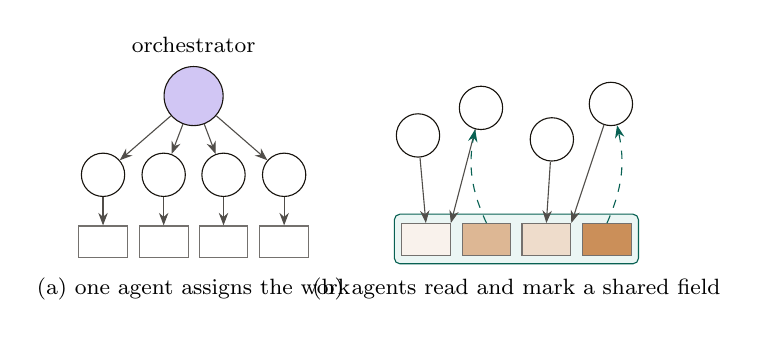
\begin{tikzpicture}[font=\footnotesize, node distance=5mm,
  ag/.style={circle,draw=ink,fill=white,minimum size=5.5mm,inner sep=0pt},
  lead/.style={circle,draw=ink,fill=lilac!35,minimum size=7.5mm,inner sep=0pt},
  part/.style={rectangle,draw=ink!60,minimum width=6.2mm,minimum height=4mm,inner sep=0pt},
  ar/.style={-{Stealth[length=1.6mm]},draw=ink!75}]
% left: orchestrator
\node[lead] (L) at (0,1.75) {};
\foreach \i/\x in {1/-1.15,2/-0.38,3/0.38,4/1.15} {
  \node[ag] (w\i) at (\x,0.75) {};
  \draw[ar] (L) -- (w\i);
  \node[part] (p\i) at (\x,-0.1) {};
  \draw[ar] (w\i) -- (p\i);
}
\node[above=0.5mm of L] {orchestrator};
\node at (0,-0.7) {(a) one agent assigns the work};
% right: field
\begin{scope}[xshift=4.1cm]
\draw[draw=teal!70!black,fill=teal!8,rounded corners=2pt] (-1.55,-0.38) rectangle (1.55,0.25);
\foreach \i/\x/\c in {1/-1.15/8,2/-0.38/45,3/0.38/22,4/1.15/70} {
  \node[part,fill=amber!\c] (q\i) at (\x,-0.07) {};
}
\foreach \i/\x/\y in {1/-1.25/1.25,2/-0.45/1.6,3/0.45/1.2,4/1.2/1.65} {
  \node[ag] (a\i) at (\x,\y) {};
}
\draw[ar] (a1) -- (q1.north);
\draw[ar] (a2) -- (q1.north east);
\draw[ar] (a3) -- (q3.north);
\draw[ar] (a4) -- (q3.north east);
\draw[ar,dashed,draw=teal!70!black] (q2.north) to[bend left=18] (a2);
\draw[ar,dashed,draw=teal!70!black] (q4.north) to[bend right=18] (a4);
\node at (0,-0.7) {(b) agents read and mark a shared field};
\end{scope}
\end{tikzpicture}
\caption{Two ways to coordinate. In (a) the picture of the work lives in one agent. In (b) it lives in the field: shading stands for marks left by earlier visits, and agents choose where to work from the marks.}
\label{fig:two}
\end{figure}

\begin{table*}[t]
\centering\small
\begin{tabularx}{\textwidth}{@{}>{\raggedright\arraybackslash}p{2.9cm} >{\raggedright\arraybackslash}p{2.2cm} >{\raggedright\arraybackslash}p{2.3cm} Y >{\raggedright\arraybackslash}p{1.6cm} >{\raggedright\arraybackslash}p{2.6cm}@{}}
\toprule
Regime & Assignment $\alpha$ & Traces used & Selection $\pi$ and kernel & Other values & Executor $x$ \\
\midrule
Orchestrator & an agent & none on the field; results return to its context & -- & -- & a model \\
Fixed schedule & a rule blind to the field & none & parts in a fixed order & -- & runtime \\
Deep agent & none ($N=1$, $b=B$) & its own working notes & -- & -- & the agent \\
\midrule
Stigmergy, avoid & the field & visit & avoid; same part & $h=\infty$ or finite & runtime \\
Stigmergy, follow & the field & change ($w>0$), visit ($w<0$) & follow; neighbouring parts & $h=\infty$ & runtime, or the agents \\
Follow with confirmation & the field & change, visit & follow; neighbouring parts & $q=2$ & runtime \\
Planned search & the field & change, visit & follow neighbours of a change; otherwise probes spaced by the size of an edit & $h=\infty$ & runtime; the plan may be written by a model \\
Threshold trigger & the field & change & continue while a change was seen in the last $k$ re-counts & $\theta$ as a stopping rule & runtime \\
\bottomrule
\end{tabularx}
\caption{Regimes as points in one space. The first three are the baselines every comparison carries; the rest coordinate through the field. Section~\ref{sec:pilot} reports which of them were run and on what.}
\label{tab:regimes}
\end{table*}

\textbf{Leaderless.} We call a regime \emph{leaderless} when no agent assigns work to another: $\alpha$ is not an agent. A fixed schedule is leaderless under this definition, and it is a baseline, not a swarm: it uses no trace. We call a regime \emph{field-coordinated} when $\alpha$ is the field, and \emph{bio-inspired} when it is field-coordinated and uses at least one primitive with a documented natural counterpart (Section~\ref{sec:atlas}). The orchestrator is the pattern most agent systems use today; in this notation it is the regime that keeps the state of the work in one context instead of on the field.

\textbf{Rule or behaviour.} The executor is a parameter and not part of the definition, because both cases exist. A selection rule can be applied by the runtime, with agents that only read and deposit; or the agents can be shown the traces and left to choose. The same regime can also be obtained in different ways: written by hand, or planned once by a model and then run as code. Which of these holds for a given result is stated with the result.

\textbf{Matched cost.} Two arms of a comparison are at matched cost when they spend the same budget $B$ in tokens as returned and priced by the provider, counting every call that plans, assigns, merges or reads the field. Equal numbers of calls or of agents are not matched cost. Elapsed time is reported as a second axis, since a collective can spend the same tokens in less time.

\subsection{Presets}

We name three regimes after the collectives that motivate them (Table~\ref{tab:presets}). The names are communication, not claims about the animals, and each preset is a hypothesis about which class of problem a setting of the primitives fits. None has been compared with the others; that comparison is the subject of a later paper.

\begin{table}[t]
\centering\small
\begin{tabularx}{\columnwidth}{@{}l Y@{}}
\toprule
Preset & Setting \\
\midrule
Ants & $\alpha$ = field; follow, local kernel. Deposit: the work product and change marks, $w>0$. Decay slow against the length of the task. $q=1$, $\rho=1$. \emph{For converging on one artefact that changes in places.} \\
Bees & Several agents explore options in parallel. Deposit: an advertisement per option, $w$ growing with assessed quality. Inhibition: objections against rival options, $w<0$. Commit at a high quorum $q$ of independent authors; fast decay, so abandoned options fade. \emph{For choosing among alternatives.} \\
Wasps & Recognition $\rho<1$ for content whose author is not recognised, which is held apart until confirmed. Low threshold $\theta$ for inspection, and inspectors recruited in proportion to the stimulus. $q \ge 2$ before a danger mark recruits. \emph{For detecting and containing what does not belong.} \\
\bottomrule
\end{tabularx}
\caption{Three presets. Numerical values are set per task. The follow regime of Table~\ref{tab:regimes} is the closest we have run to Ants, and follow with confirmation uses one element of Wasps; Bees has not been run.}
\label{tab:presets}
\end{table}

\section{An atlas of swarming species}\label{sec:atlas}

Table~\ref{tab:atlas} maps eight collectives to a mechanism, to the primitives it involves and to a class of problem. A collective enters the atlas when four conditions hold: it is a population of units of the same kind; no unit directs the others; coordination happens through local interaction or through the environment; and a primary source quantifies the mechanism. The rule leaves out much of what inspired the programme (immune responses, organs, analogies from physics), which stays as motivation for other hypotheses, and one of the nine plates of the public Atlas of Swarms: for the bait ball of sardines we hold no verified source.

The class-of-problem column is stated in terms of what a task asks of a group: which share of the field the budget can read, whether the field changes during the work, whether traces say where to look next, and whether a claim can be checked more cheaply than it is produced. Each entry in that column is a hypothesis.

The last column is the evidence we hold for the engineering analogue with language-model agents, and it is the point of the table. Four rows have any, and in each it is partial: a mechanism supported under stated conditions, or tested in one of its forms. For the rest the analogue is a hypothesis, in one case with support inside a simulation only. The atlas is a map of what to test, not of what works.

\begin{table*}[t]
\centering\small
\begin{tabularx}{\textwidth}{@{}l >{\raggedright\arraybackslash}p{1.75cm} >{\raggedright\arraybackslash}p{3.3cm} >{\raggedright\arraybackslash}p{1.9cm} Y >{\raggedright\arraybackslash}p{4.1cm}@{}}
\toprule
 & Collective & Mechanism & Primitives & Class of problem (hypothesis) & Evidence for the analogue with language-model agents \\
\midrule
I & Starlings & each bird tracks a fixed number of nearest neighbours~\cite{ballerini2008} & none of the five: a bound on what each agent reads & keeping many agents consistent at bounded reading cost & none \\
II & Desert locusts & crowding flips individuals into collective motion & threshold & deciding when solitary work should become collective & stopping by threshold rules against a model that decides (Section~\ref{sec:pilot}); readers simulated \\
III & Honey bees & scouts recruit in proportion to quality, inhibit rivals, commit at a quorum~\cite{seeley2003,seeley2012} & deposit, inhibition, quorum & choosing among alternatives when each evaluation is noisy & quorum as a stopping rule matched seven votes with two agents; one deeper agent was above it. Unequal options and inhibition: untested \\
IV & Fireflies & coupled oscillators synchronise & deposit (a signal) & agreeing on timing without a clock & none \\
V & Black garden ants & reinforced trails that evaporate~\cite{goss1989,dorigo1996} & deposit, decay & placing effort on a field larger than the budget, and moving it when the field changes & deposit: supported when change is local, reversed when it is scattered or a trace is false. Decay: supported as a discount on old counts, not as fading marks \\
VI & Termites & the structure built so far stimulates the next act of building~\cite{grasse1959} & deposit (the work product) & building one artefact incrementally without assigning parts & one run on a public benchmark (Section~\ref{sec:cooperbench}): a shared remote recovered part of the loss that messaging leaves, below one agent \\
VII & Slime mould & tubes that carry flow thicken, the others decay~\cite{tero2010} & deposit, decay & pruning who reads whom & in a simulation only \\
IX & Luminous bacteria & collective behaviour above a concentration of signal~\cite{miller2001} & threshold, quorum & acting only when enough independent signals accumulate & requiring a second count before a change recruits repaired a false trace (Section~\ref{sec:pilot}) \\
\bottomrule
\end{tabularx}
\caption{Atlas. Numbering follows the plates of the public Atlas of Swarms; plate VIII is left out by the inclusion rule. The last column refers to the runs reported or cited in Section~\ref{sec:pilot}.}
\label{tab:atlas}
\end{table*}

\section{Related work}\label{sec:related}

Every statement in this section was checked against the paper itself; Table~\ref{tab:related} summarises it.

\textbf{Coordination through a shared artefact.} A small recent literature has language-model agents coordinate through traces instead of messages. Rodriguez has agents patch the high-pressure regions of a shared artefact, with a fitness that decays; the pressure-field arm solves 48.5\% of scheduling problems against 11.1\% for a conversation baseline~\cite{rodriguez2026}. It spends 617 thousand tokens per trial against 38 to 46 thousand for the single-stream arms, on easy problems one agent on the field does as well as four, and the decay ablation is 29 of 30 against 26 of 30 ($p=0.35$), which the author reports as not significant. Pal et al.\ let agents build on persistent artefacts in a simulated world and compare shared worlds with isolated one-agent worlds at matched model calls~\cite{pal2026}; the lifetime of a trace is not varied. Jones and Hauert give three stateless agents a shared store whose entries decay, and state that the design does not isolate decay as the cause of what they observe~\cite{jones2026}. Buehler applies deposited cues to music composition, with one composition per system and no ablation~\cite{buehler2025}.

The closest work in mechanism is ScaleMAS~\cite{qi2026}: asynchronous agents interact only through an append-only store of linked messages, in which a message gains weight each time a later one cites it and all weights decay at every step, and a read returns the few messages ranked highest. This is deposit, reinforcement and decay on a shared field, without the biological vocabulary. The paper ablates the citation weight, scales groups to 128 agents, removes agents during a run, and compares with orchestrator, debate and blackboard systems; with four agents the shared store reaches 55.1\% on a deep-research benchmark against 38.0\% for the same agents working independently. It tests one configuration of the mechanism, and has no arm in which one agent holds the budget of the group. Reinforcement with decay on a shared store is therefore not new here; what we add is a notation in which that system, its baselines and other regimes are points of one space, and a comparison that includes the schedule and the single agent.

\textbf{Collectives against single agents.} Whether a collective beats one agent given the same resources is now asked directly. Fan et al.\ define the gain of collaboration as the performance of the collective over that of the best single agent ``allocated a total resource budget equivalent'' to it~\cite{fan2026}, and report it on small samples without intervals; our standard is theirs, with the unit fixed to tokens and uncertainty reported. Kim et al.\ compare a single agent with four message-passing architectures over 260 configurations, with outcomes from $+80.8\%$ to $-70.0\%$ depending on the task and a mean change near zero~\cite{kim2025}; the paper describes its matching both as equal iterations and as equal reasoning tokens. Gao et al.\ run a cost-matched single agent against a hierarchy under one orchestrator on four tasks, and the hierarchy is ahead on three~\cite{gao2026}; cost is in dollars and the hierarchy draws on several models. On real repositories, Khatua et al.\ find that two agents who each implement one feature and can exchange messages succeed far less often than one agent implementing both: 0.28 against 0.48 for one frontier model and 0.26 against 0.47 for another, with messaging making no difference to success~\cite{khatua2026}. None of these collectives is coordinated through a field; all use messages or an orchestrator.

\textbf{Swarm intelligence.} Ant colony optimisation and its relatives~\cite{dorigo1996} use the same natural mechanisms for numerical optimisation with simple agents, and swarm robotics studies them in embodied collectives, where decentralisation is given by the problem and a single stronger agent is not a competitor. Ruan et al.\ place language models as decentralised agents on a grid, with local messages and no shared trace, and name stigmergy as the missing piece~\cite{ruan2025}. Our agents are language models, each able to do much of the task alone, which is why the single-agent control decides.

\textbf{What is left untested.} On our reading, no work compares several field-coordinated regimes with each other on one task; none compares a field-coordinated collective with a fixed schedule; and where a mechanism was ablated, the effect was either not significant or tested in one configuration. The comparison with one agent at equal budget exists for message-passing and orchestrated systems and not for a leaderless, field-coordinated one. The pilot of Section~\ref{sec:pilot} makes those comparisons on a small scale; it matches arms in reads and reports tokens, which is weaker than the standard we state.

\begin{table*}[t]
\centering\small
\begin{tabularx}{\textwidth}{@{}>{\raggedright\arraybackslash}p{3.4cm} >{\raggedright\arraybackslash}p{2.4cm} Y >{\raggedright\arraybackslash}p{3.0cm} >{\raggedright\arraybackslash}p{3.3cm}@{}}
\toprule
Work & Coordination through a shared field & One agent with the budget of the collective & Field regimes compared with each other & Mechanism ablated \\
\midrule
Pressure fields~\cite{rodriguez2026} & yes & no; tokens reported, 4 to 16 times apart & no & decay: not significant \\
SwarmWorld~\cite{pal2026} & yes & no; isolated agents at matched calls & layers on one substrate & no \\
Emergent culture~\cite{jones2026} & yes & no task & no & no \\
MusicSwarm~\cite{buehler2025} & yes & no & no & no \\
ScaleMAS~\cite{qi2026} & yes & no & no; ranking rule varied & citation weight \\
SwarmBench~\cite{ruan2025} & no; local messages & no & no & parameters swept \\
SwarmBench~\cite{gao2026} & no; orchestrator & yes, in dollars, four tasks & -- & -- \\
Scaling agent systems~\cite{kim2025} & no; messages & yes; unit stated two ways & -- & -- \\
Collective AI~\cite{fan2026} & no & yes, in tokens; defines the standard & -- & -- \\
CooperBench~\cite{khatua2026} & no; messages & equal workload; no token accounting & -- & messaging on and off \\
\midrule
This paper (pilot) & yes & equal reads; tokens reported, not equal & yes & decay: not significant; confirmation \\
\bottomrule
\end{tabularx}
\caption{What neighbouring work tests, read from the papers.}
\label{tab:related}
\end{table*}

\section{Pilot}\label{sec:pilot}

The pilot applies the standard of Section~\ref{sec:framework} to one synthetic task in four settings. It is small on purpose: it shows what the comparison looks like when every arm is a point of Table~\ref{tab:regimes} and the baselines are present, and it reports what happened, including where the field-coordinated regimes lost. Each setting was preregistered before its first paid call; the runs are listed in Appendix~\ref{app:runs}.

\subsection{Design}

\textbf{Task.} A collection of 288 synthetic study records by six authors is split into parts. The answer is the author with the most studies that are peer-reviewed, from 2020 or later and positive: 20 for the leader and 16 for the runner-up. An agent reads one part (in setting A, at most two) and returns a count per author; the answer is computed by code from the latest count of each part. Every collection is run in a \emph{stable} condition, in which nothing changes, and an \emph{edited} condition, in which the collection is edited silently part-way through so that the answer reverses. No agent is told. All agents are Claude Haiku~5.5 with reasoning disabled and 80 words of working space; an orchestrator, where there is one, is the same model.

\textbf{Settings.}
\emph{A, full coverage}: six parts of 48 records; the budget reads every part twice; one part is edited after the first pass. Thirty collections.
\emph{B, partial coverage, local change}: twelve parts of 24 records in a ring; every part is counted once and the budget then allows six re-counts, in three rounds of two; three neighbouring parts are edited. Sixty collections.
\emph{C, scattered change}: as B, with three edited parts no two of which are neighbours. Sixty collections.
\emph{D, a false trace}: as B, with one false count placed on the board before the re-counts. Sixty collections.
In B, C and D the answer is right only if at least two of the three edited parts are re-counted.

\textbf{Regimes.} The arms are the regimes of Table~\ref{tab:regimes}. The fixed schedule re-reads parts in order. The deep agent is, in A, the same schedule in half as many calls with twice the working space, and in B and C a single agent that makes all six re-counts in sequence, seeing the board and choosing its next part each time. The orchestrator reads the board each round and assigns the readers; in B, C and D it is told that an edit tends to affect neighbouring parts. \emph{Stigmergy, avoid}: readers go to parts with the weakest visit marks, with marks that halve every round or never fade. \emph{Stigmergy, follow}: a count that differs from the previous count of its part leaves a change mark, and readers are drawn to the neighbours of a change mark and away from parts already re-read. \emph{Follow with confirmation} re-counts a marked part once before its neighbours are visited. In all field-coordinated arms the rule is applied by the runtime.

Within a setting every arm makes the same number of reads; cost in tokens is reported per arm and is not equal across arms. Predictions were on accuracy in the edited condition, paired by collection, with 95\% bootstrap intervals.

\subsection{Results}

In the stable condition every regime was right on every collection in every setting. Table~\ref{tab:results} and Figure~\ref{fig:results} give the edited condition.

\begin{table*}[t]
\centering\small
% generated by make-figures.mjs; do not edit
\begin{tabular}{@{}lcccc@{}}
\toprule
Regime & A: full coverage & B: partial, local & C: partial, scattered & D: partial, false trace \\
 & $n=30$ & $n=60$ & $n=60$ & $n=60$ \\
\midrule
Fixed schedule & 30 (1.00) & 29 (0.48) & 28 (0.47) & 23 (0.38) \\
Deep agent & 30 (1.00) & 45 (0.75) & 21 (0.35) & -- \\
Orchestrator & 30 (1.00) & 45 (0.75) & 12 (0.20) & 16 (0.27) \\
Stigmergy, avoid, with decay & 17 (0.57) & -- & -- & -- \\
Stigmergy, avoid, no decay & 18 (0.60) & -- & -- & -- \\
Stigmergy, follow & -- & 42 (0.70) & 17 (0.28) & 10 (0.17) \\
Follow with confirmation & -- & -- & -- & 22 (0.37) \\
\bottomrule
\end{tabular}

\caption{Collections right in the edited condition, as a count and a share. Dashes are arms that were not run in a setting. Generated from the result files by \texttt{make-figures.mjs}.}
\label{tab:results}
\end{table*}

\begin{figure*}[t]
\centering
% generated by make-figures.mjs; do not edit
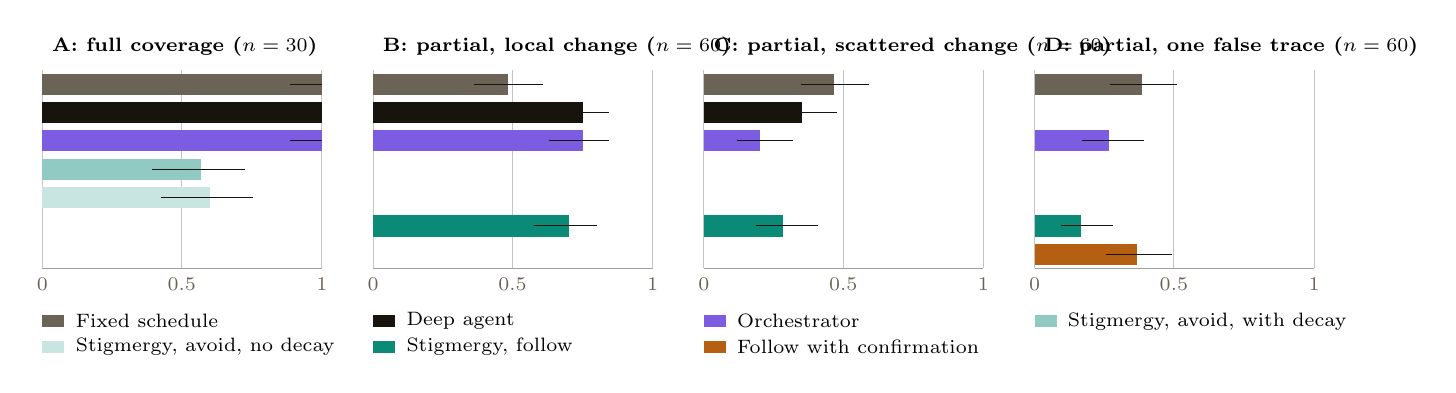
\begin{tikzpicture}[font=\scriptsize]
\begin{scope}[xshift=0.00cm]
\node[anchor=south west,font=\scriptsize\bfseries] at (0,2.57) {A: full coverage ($n=30$)};
\draw[draw=ink!40] (0,0) -- (3.55,0);
\draw[draw=ink!25] (0.00,0) -- (0.00,2.52); \node[anchor=north,text=mute] at (0.00,0) {0};
\draw[draw=ink!25] (1.77,0) -- (1.77,2.52); \node[anchor=north,text=mute] at (1.77,0) {0.5};
\draw[draw=ink!25] (3.55,0) -- (3.55,2.52); \node[anchor=north,text=mute] at (3.55,0) {1};
\fill[mute] (0,2.205) rectangle (3.550,2.475);
\draw[draw=ink,line width=0.4pt] (3.147,2.340) -- (3.550,2.340);
\fill[ink] (0,1.845) rectangle (3.550,2.115);
\draw[draw=ink,line width=0.4pt] (3.147,1.980) -- (3.550,1.980);
\fill[lilac] (0,1.485) rectangle (3.550,1.755);
\draw[draw=ink,line width=0.4pt] (3.147,1.620) -- (3.550,1.620);
\fill[teal!45] (0,1.125) rectangle (2.012,1.395);
\draw[draw=ink,line width=0.4pt] (1.392,1.260) -- (2.578,1.260);
\fill[teal!22] (0,0.765) rectangle (2.130,1.035);
\draw[draw=ink,line width=0.4pt] (1.502,0.900) -- (2.677,0.900);
\end{scope}
\begin{scope}[xshift=4.20cm]
\node[anchor=south west,font=\scriptsize\bfseries] at (0,2.57) {B: partial, local change ($n=60$)};
\draw[draw=ink!40] (0,0) -- (3.55,0);
\draw[draw=ink!25] (0.00,0) -- (0.00,2.52); \node[anchor=north,text=mute] at (0.00,0) {0};
\draw[draw=ink!25] (1.77,0) -- (1.77,2.52); \node[anchor=north,text=mute] at (1.77,0) {0.5};
\draw[draw=ink!25] (3.55,0) -- (3.55,2.52); \node[anchor=north,text=mute] at (3.55,0) {1};
\fill[mute] (0,2.205) rectangle (1.716,2.475);
\draw[draw=ink,line width=0.4pt] (1.284,2.340) -- (2.155,2.340);
\fill[ink] (0,1.845) rectangle (2.662,2.115);
\draw[draw=ink,line width=0.4pt] (2.228,1.980) -- (2.990,1.980);
\fill[lilac] (0,1.485) rectangle (2.662,1.755);
\draw[draw=ink,line width=0.4pt] (2.228,1.620) -- (2.990,1.620);
\fill[teal] (0,0.405) rectangle (2.485,0.675);
\draw[draw=ink,line width=0.4pt] (2.041,0.540) -- (2.844,0.540);
\end{scope}
\begin{scope}[xshift=8.40cm]
\node[anchor=south west,font=\scriptsize\bfseries] at (0,2.57) {C: partial, scattered change ($n=60$)};
\draw[draw=ink!40] (0,0) -- (3.55,0);
\draw[draw=ink!25] (0.00,0) -- (0.00,2.52); \node[anchor=north,text=mute] at (0.00,0) {0};
\draw[draw=ink!25] (1.77,0) -- (1.77,2.52); \node[anchor=north,text=mute] at (1.77,0) {0.5};
\draw[draw=ink!25] (3.55,0) -- (3.55,2.52); \node[anchor=north,text=mute] at (3.55,0) {1};
\fill[mute] (0,2.205) rectangle (1.657,2.475);
\draw[draw=ink,line width=0.4pt] (1.229,2.340) -- (2.098,2.340);
\fill[ink] (0,1.845) rectangle (1.242,2.115);
\draw[draw=ink,line width=0.4pt] (0.858,1.980) -- (1.691,1.980);
\fill[lilac] (0,1.485) rectangle (0.710,1.755);
\draw[draw=ink,line width=0.4pt] (0.420,1.620) -- (1.128,1.620);
\fill[teal] (0,0.405) rectangle (1.006,0.675);
\draw[draw=ink,line width=0.4pt] (0.657,0.540) -- (1.447,0.540);
\end{scope}
\begin{scope}[xshift=12.60cm]
\node[anchor=south west,font=\scriptsize\bfseries] at (0,2.57) {D: partial, one false trace ($n=60$)};
\draw[draw=ink!40] (0,0) -- (3.55,0);
\draw[draw=ink!25] (0.00,0) -- (0.00,2.52); \node[anchor=north,text=mute] at (0.00,0) {0};
\draw[draw=ink!25] (1.77,0) -- (1.77,2.52); \node[anchor=north,text=mute] at (1.77,0) {0.5};
\draw[draw=ink!25] (3.55,0) -- (3.55,2.52); \node[anchor=north,text=mute] at (3.55,0) {1};
\fill[mute] (0,2.205) rectangle (1.361,2.475);
\draw[draw=ink,line width=0.4pt] (0.962,2.340) -- (1.810,2.340);
\fill[lilac] (0,1.485) rectangle (0.947,1.755);
\draw[draw=ink,line width=0.4pt] (0.608,1.620) -- (1.385,1.620);
\fill[teal] (0,0.405) rectangle (0.592,0.675);
\draw[draw=ink,line width=0.4pt] (0.331,0.540) -- (0.995,0.540);
\fill[amber] (0,0.045) rectangle (1.302,0.315);
\draw[draw=ink,line width=0.4pt] (0.910,0.180) -- (1.751,0.180);
\end{scope}
\begin{scope}[yshift=-0.75cm]
\fill[mute] (0,0) rectangle +(0.28,0.16); \node[anchor=west] at (0.3,0.08) {Fixed schedule};
\fill[ink] (4.2,0) rectangle +(0.28,0.16); \node[anchor=west] at (4.5,0.08) {Deep agent};
\fill[lilac] (8.4,0) rectangle +(0.28,0.16); \node[anchor=west] at (8.700000000000001,0.08) {Orchestrator};
\fill[teal!45] (12.600000000000001,0) rectangle +(0.28,0.16); \node[anchor=west] at (12.900000000000002,0.08) {Stigmergy, avoid, with decay};
\fill[teal!22] (0,-0.33) rectangle +(0.28,0.16); \node[anchor=west] at (0.3,-0.25) {Stigmergy, avoid, no decay};
\fill[teal] (4.2,-0.33) rectangle +(0.28,0.16); \node[anchor=west] at (4.5,-0.25) {Stigmergy, follow};
\fill[amber] (8.4,-0.33) rectangle +(0.28,0.16); \node[anchor=west] at (8.700000000000001,-0.25) {Follow with confirmation};
\end{scope}
\end{tikzpicture}

\caption{Share of collections right in the edited condition, with 95\% Wilson intervals.}
\label{fig:results}
\end{figure*}

\textbf{A. With full coverage a fixed schedule is enough.} The three arms that re-read every part were right on 30 of 30. Undirected stigmergy re-read the edited part in 60 to 70\% of collections and was right on 17 and 18 of 30: the schedule was ahead by 0.43 (0.27 to 0.60), as the design implies when the budget allows a full sweep. The orchestrator reproduced the sweep, covering 5.6 distinct parts of six in its second pass, at 11\% more cost. Decay made no difference: 17 against 18 of 30 ($-0.03$; $-0.27$ to [US$ redacted]$), a sample too small to detect the 0.13 the schedules predict with error-free readers. The schedule, the deep agent and the orchestrator are at ceiling and cannot be separated here.

\textbf{B. Under partial coverage with local change, following traces beats the schedule.} The follow regime was right on 0.70 of collections against 0.48 for the fixed schedule ($+0.22$; 0.05 to 0.38), the second of two independent runs with the same outcome. Given the same marks, the orchestrator reached 0.75, not distinguishable from the rule ($+0.05$; $-0.10$ to [US$ redacted]$), at 16\% more cost. One agent holding the whole re-count budget also reached 0.75: above the schedule ($+0.27$; 0.12 to 0.42) and equal to the orchestrator with two readers ([US$ redacted]$; $-0.15$ to [US$ redacted]$).

\textbf{C and D. The same rule loses when its assumption fails.} With scattered edits the follow regime fell to 0.28 against 0.47 for the schedule ($-0.18$; $-0.37$ to [US$ redacted]$). The orchestrator, given the same assumption in words, fell further, to 0.20 ($-0.27$ against the schedule; $-0.43$ to $-0.10$), and the single agent to 0.35 ($-0.12$; $-0.27$ to [US$ redacted]$). With one false count on the board the follow regime fell to 0.17 against 0.38 ($-0.22$; $-0.37$ to $-0.07$): it spent 2.5 of its six re-counts beside the false mark. Requiring a second count before a mark recruits brought it back to 0.37 ($+0.20$ over the unconfirmed rule; 0.05 to 0.35), level with the schedule and not above it.

\textbf{Cost.} The four settings cost US\$\,0.59, 1.22, and 1.93 (C and D together) in model usage at list prices, for about 22,500 requests in all. The arms of a setting are matched in the number of reads, not in tokens, so by the definition of Section~\ref{sec:framework} they are close to matched cost and not at it. The orchestrator cost 11 to 19\% more than the fixed schedule in every setting. The single agent of settings B and C cost 37\% more than the schedule (US\$\,0.30 against 0.22 per setting), because it reads the board again at every step; in setting A the deep agent cost 15\% less. The follow regime cost the same as the schedule, so its advantage in B and its losses in C and D are at matched cost. The orchestrator and the single agent spent more than the schedule they beat in B, and those two comparisons are confounded with cost.

\subsection{What the pilot shows}

Three statements are supported, each on one task and one small model. First, when the budget covers the field, coordination through traces has nothing to add to a schedule, and neither has an orchestrator. Second, when it does not and change is local, a trace on the field and a rule that follows it beat the best schedule; whether the rule is applied by the runtime, by an orchestrator or by one agent working alone made no measurable difference. Third, the gain is conditional: the rule is a bet on how the field changes, every arm that made the bet lost it under scattered change, and a trace that is not confirmed can be turned against the regime that trusts it.

What the pilot does not show matters as much. No field-coordinated regime was above a single agent with the same budget. Decay had no measurable effect at this sample; a larger run outside the pilot, below, found one. Quorum appears only as confirmation of a trace, and recognition does not appear. The task is a count over a few hundred records, which one agent with enough working space can do alone.

\subsection{Runs outside the pilot}

Six further preregistered runs bear on the framework and are reported in the repository, not here, because they were designed after the pilot's results were seen. When readers were shown the marks and chose for themselves, they went to a fresh neighbour of a change in 90\% of choices and almost never explored, ending between the schedule and the runtime rule. A larger model given the locality assumption planned a search that was right on 0.98 of collections in setting B; written as a rule, the same search is exact in simulation and is the planned search of Table~\ref{tab:regimes}. A model asked after each round whether to keep re-counting stopped early and was 0.20 below the best threshold rule. And a model that plans once from a single example chose the right rule for a field whose structure it was not told, within 0.03 of the best rule of a family of 85. The last three used simulated readers or a second model and are exploratory. Two runs tested primitives the pilot leaves thin. \emph{Decay}: on 150 collections of setting A, avoid-stigmergy was right on 0.67 with decay against 0.41 without ($+0.26$; 0.17 to 0.35), at a cost of 0.03 to 0.05 when nothing had changed; re-estimating the same reads shows that the whole effect comes from discounting old counts when they are combined ($+0.28$) and none from the fading of visit marks ($-0.02$). The 30 collections of the pilot were too few to see it. \emph{Quorum}: on 300 tasks in each of two task families, stopping at the second matching answer gave the accuracy of seven votes with 2.2 agents, and seven votes were 0.04 above one agent; one agent with three times the working space was above the quorum at a third of its tokens.

\subsection{A run on a public benchmark}\label{sec:cooperbench}

The pilot's task is ours. To see one row of the atlas on a task that is not, we ran the benchmark of Khatua et al.~\cite{khatua2026} with its own harness and code, on the maintainers' subset of 50 feature pairs from 20 tasks in 11 repositories, with the same small model. A pair counts when the hidden tests of both features pass on the merged result. Four arms were registered before the run: one agent implementing both features; two agents with no communication; two agents with messaging; and two agents with no messaging and a shared remote to which each pushes and from which each can fetch and merge the other's work, which is the benchmark's own shared-artefact mode and the nearest existing thing to row~VI of Table~\ref{tab:atlas}. Intervals resample the 20 tasks.

One agent delivered 29 of 50 pairs. Two agents with no communication delivered 8, with messaging 10, and with the shared remote 19. The shared remote was above messaging by 0.18 (0.07 to 0.32) and above no communication by 0.22 (0.10 to 0.37); every pair delivered in either of those arms was also delivered with the remote. Messaging was not distinguishable from no communication ($+0.04$; 0.00 to 0.12) and cost 44\% more. The loss is a merge problem: without communication 34 of 50 pairs ended in a merge conflict, with messaging 28, with the shared remote 23, and the remote also raised the share of clean merges that pass. No cooperating arm was above one agent: the best was 0.20 below it ($-0.37$ to [US$ redacted]$), at more than twice the cost (US\$\,2.24 against 0.99).

Two things follow, and one does not. A visible, shared work product removed part of a coordination loss that conversation left in place, on real code, which is what the stigmergy row predicts. It recovered about half of the distance to a single agent and not more. It does not show a collective ahead of one agent, because on these tasks one agent is better than two under every medium tried; and it does not show that agents take up such a medium unprompted, since the benchmark's prompt for this mode tells them to push, fetch and merge. The run is one pass per pair with one model; two pairs of the shared-remote arm had no result after the one registered rerun and are counted as failures.

\section{Discussion}

\textbf{Where a collective is expected to pay.} The pilot varies one property of the task at a time, and the outcome follows it. When the budget reads the whole field, nothing coordinated through traces improved on a schedule. When it reads half and change is local, a trace and a rule that follows it did. When change is scattered, or a trace is false, the same rule lost to the schedule. We read these as the first entries of a map from properties of a task to the regime that fits it: the share of the field the budget can read, whether the field changes during the work, whether traces say where to look next, and whether a trace can be checked. Two further properties are not in the pilot and are where the case for a collective is usually made: a task that exceeds what one agent can hold, and members that fail. On a task one agent can hold, our own runs outside this paper found one agent with room to reason above every collective of agents with less.

\textbf{What the leader contributed.} In no setting did an orchestrator do better than a rule given the same information, and it cost more in each. Under full coverage it reproduced the schedule; under local change it matched the follow rule; under scattered change it followed the assumption it had been given and did worse than the rule. The supported statement is narrower than ``leaderless is better'': on this task the state of the work could sit on the field instead of in one context at no loss, and what decided the outcome was the policy, not who held it. A stronger orchestrator found a better policy, which then ran as a rule.

\textbf{Rule or behaviour.} In the pilot every field-coordinated rule is applied by the runtime, and the agents only read and deposit. That makes the rule exact and repeatable, and it is a model of stigmergy more than a swarm of agents that practise it. When the agents were shown the marks and chose, they responded to a change as the rule does and did not explore; told why exploration matters, they explored, with no measurable gain. Whether a regime should live in the runtime, in the agents, or be planned once and compiled is open, and the framework treats it as a parameter so that the three can be compared.

\textbf{What would refute the framework.} The framework is useful if regimes written in it can be compared and if the primitives carry the differences. It fails if a field-coordinated regime cannot be distinguished from its schedule baseline once cost is matched across the tasks where traces should matter; or if the differences between regimes are carried by something the notation leaves out, such as the working space of each agent, which was the largest effect in our other runs. Recognition has no evidence here with language-model agents; threshold and quorum have it only as stopping rules; and decay, the primitive most often claimed, turned out to matter as a discount on old evidence and not as the evaporation of a trail.

\textbf{The human as a perturbation.} The silent edit of the pilot is an intervention on the field from outside. In a leaderless system that is the natural form of human control: the operator does not command an agent, but changes what the agents read. The false trace of setting D is the same act with a different intent, and the regime that trusted traces without confirmation was the one it defeated. We leave the study of the operator to later work.

\section{Limitations}

The task is synthetic and its answer is a count; one agent with enough working space can do it alone, so the pilot cannot show a collective exceeding what one agent can do. Thirty or sixty collections give intervals of 0.15 to 0.2 on a difference. One provider and one small model, with reasoning disabled, were used for all agents. Arms are matched in reads and not in tokens, and two of the comparisons are confounded with cost as stated. The rules are applied by the runtime. The structure of change (local, scattered) was chosen by us, and a regime's fit to it is by construction. The biological mechanisms are analogies; simulation results quoted as motivation are support inside a model. The atlas's class-of-problem column is a set of hypotheses. The benchmark run of Section~\ref{sec:cooperbench} is one pass on 50 pairs with one small model and two agents, its arms are not matched in cost, and its shared-remote arm uses a prompt written by the benchmark's maintainers. Beyond that run, nothing here supports a claim about coding, research or defensive work.

\section{Conclusion}

We proposed a vocabulary in which an orchestrator, a schedule, a single deep agent and a bio-inspired swarm can be written side by side, an atlas that connects swarming species to the problems their mechanisms address, and a standard for comparing them. In a pilot on one synthetic task, coordination through traces beat a fixed schedule only when the budget did not cover the field and change was local, lost when that assumption failed, and at no point exceeded one agent with the same budget; an orchestrator added nothing a rule did not. On a public benchmark of real repositories a shared work product recovered about half of the loss that two agents suffer against one, where messaging recovered almost none. The work is a first step towards bio-inspired and leaderless AI swarms; the next asks, across tasks and at matched cost, when such swarms beat an orchestrator.

{\small
\begin{thebibliography}{99}\setlength{\itemsep}{0.15em}
\bibitem{grasse1959} P.-P. Grass\'e. La reconstruction du nid et les coordinations interindividuelles chez \emph{Bellicositermes natalensis} et \emph{Cubitermes} sp. \emph{Insectes Sociaux}, 6:41--80, 1959.
\bibitem{theraulaz1999} G. Theraulaz and E. Bonabeau. A brief history of stigmergy. \emph{Artificial Life}, 5(2):97--116, 1999.
\bibitem{goss1989} S. Goss, S. Aron, J.-L. Deneubourg, and J. M. Pasteels. Self-organized shortcuts in the Argentine ant. \emph{Naturwissenschaften}, 76:579--581, 1989.
\bibitem{dorigo1996} M. Dorigo, V. Maniezzo, and A. Colorni. Ant system: optimization by a colony of cooperating agents. \emph{IEEE Trans.\ Systems, Man, and Cybernetics B}, 26(1):29--41, 1996.
\bibitem{bonabeau1996} E. Bonabeau, G. Theraulaz, and J.-L. Deneubourg. Quantitative study of the fixed threshold model for the regulation of division of labour in insect societies. \emph{Proc.\ R.\ Soc.\ B}, 263:1565--1569, 1996.
\bibitem{seeley2003} T. D. Seeley and P. K. Visscher. Choosing a home: how the scouts in a honey bee swarm perceive the completion of their group decision making. \emph{Behavioral Ecology and Sociobiology}, 54:511--520, 2003.
\bibitem{seeley2012} T. D. Seeley et al. Stop signals provide cross inhibition in collective decision-making by honeybee swarms. \emph{Science}, 335:108--111, 2012.
\bibitem{miller2001} M. B. Miller and B. L. Bassler. Quorum sensing in bacteria. \emph{Annual Review of Microbiology}, 55:165--199, 2001.
\bibitem{ballerini2008} M. Ballerini et al. Interaction ruling animal collective behavior depends on topological rather than metric distance. \emph{PNAS}, 105(4):1232--1237, 2008.
\bibitem{tero2010} A. Tero et al. Rules for biologically inspired adaptive network design. \emph{Science}, 327:439--442, 2010.
\bibitem{rodriguez2026} R. R. Rodriguez, Jr. Emergent coordination in multi-agent systems via pressure fields and temporal decay. arXiv:2601.08129v3, 2026.
\bibitem{pal2026} S. Pal, F. Y. Wang, and M. J. Buehler. SwarmWorld: stigmergic technological evolution in societies of language-model agents. arXiv:2608.26081v1, 2026.
\bibitem{jones2026} S. Jones and S. Hauert. Emergent culture in minimal LLM systems. arXiv:2606.30668v1, 2026.
\bibitem{buehler2025} M. J. Buehler. MusicSwarm: biologically inspired intelligence for music composition. arXiv:2509.11973v1, 2025.
\bibitem{qi2026} Z. Qi et al. Scaling multi-agent intelligence with substrate-centric coordination. arXiv:2610.16120v1, 2026.
\bibitem{fan2026} J. Fan et al. Towards a science of collective AI: LLM-based multi-agent systems need a transition from blind trial-and-error to rigorous science. arXiv:2602.05289v1, 2026.
\bibitem{kim2025} Y. Kim et al. Towards a science of scaling agent systems. arXiv:2512.08296v3, 2026.
\bibitem{gao2026} J. Gao, Z. Jin, T. Men, K. Liu, and J. Zhao. SwarmBench: can large language models act as agent swarm orchestrators? arXiv:2608.30661v1, 2026.
\bibitem{khatua2026} A. Khatua et al. CooperBench: why coding agents cannot be your teammates yet. arXiv:2601.13295v2, 2026.
\bibitem{ruan2025} K. Ruan, M. Huang, J.-R. Wen, and H. Sun. Benchmarking LLMs' swarm intelligence. arXiv:2505.04364v4, 2025.
\end{thebibliography}
}


\appendix
\section{Runs, preregistrations and reproduction}\label{app:runs}

Every run was registered before its first paid call, frozen by a hash of its code and requests, and submitted once. Table~\ref{tab:runs} lists the runs behind Section~\ref{sec:pilot}. Paths are relative to the laboratory's research repository, to be released with the paper; each report states its own limits. The table and figure of Section~\ref{sec:pilot} are generated from the result files by \texttt{make-figures.mjs}, and the differences and intervals quoted in the text are those of the reports.

\begin{table*}[t]
\centering\small
\begin{tabularx}{\textwidth}{@{}>{\raggedright\arraybackslash}p{4.2cm} Y r r@{}}
\toprule
Run & Report (under \texttt{results/}); its first lines name the preregistration & Requests & US\$ \\
\midrule
Setting A (five regimes) & \texttt{batch2-r1-regimes/REPORT.md} & 2,550 & 0.59 \\
Setting B (four arms) & \texttt{batch2-r2b-regimes/REPORT.md} & 6,060 & 0.92 \\
Settings C and D & \texttt{batch2-r3-bounds/REPORT.md} & 10,800 & 1.63 \\
Single agent in B and C & \texttt{batch2-d6-deep/REPORT.md} & 3,120 & 0.60 \\
\midrule
Agents choosing from marks & \texttt{batch2-d4-choice/REPORT.md}, \texttt{batch2-d4b-choice/REPORT.md} & & \\
Orchestrator model and prior & \texttt{ring-routers/REPORT.md} & & \\
Stopping as a decision & \texttt{batch2-t1-trigger/REPORT.md} & & \\
Planning a rule from examples & \texttt{batch2-pd1-policy/REPORT.md} & & \\
Decay at three rates & \texttt{batch2-d5-decay/REPORT.md} & 8,100 & 1.82 \\
Quorum as a stopping rule & \texttt{batch2-q1-quorum/REPORT.md} & 5,400 & 0.92 \\
Public benchmark, four arms & \texttt{cb2-cooperbench/REPORT.md} & 200 pair runs & 6.45 \\
\bottomrule
\end{tabularx}
\caption{Runs of the pilot (above the rule) and runs outside it that the text cites (below). Costs are model usage at list prices estimated from returned tokens, not invoices; the benchmark row is the cost its harness reports.}
\label{tab:runs}
\end{table*}

The laboratory's consolidated table of its runs records eight corrections to its own earlier statements. Three bear on this paper: an orchestrator result withdrawn because the task generator leaked the location of the edit; the statement that decay had no effect, replaced by the larger run cited in Section~\ref{sec:pilot}; and the statement that a vote among reasoning agents adds nothing, softened to a gain of 0.01 to 0.04 at three to seven times the tokens.

\end{document}
